\documentclass{article} % For LaTeX2e
\usepackage{iclr2026_conference,times}
% Optional math commands from https://github.com/goodfeli/dlbook_notation.
\input{math_commands.tex}
\usepackage{hyperref}
\usepackage{url}
\usepackage{graphicx}
\usepackage{booktabs}
\usepackage{amsmath}
\graphicspath{{../out/presentation_figs/}}

\title{Incremental Structure from Motion: \\ A Three-Image Pipeline Scaled to Multi-View Reconstruction}

\author{Group 5: yhl63, ri302, jp2057}

\iclrfinalcopy % Uncomment for camera-ready version, but NOT for submission.

\begin{document}
\maketitle

\begin{abstract}
We present an incremental Structure-from-Motion (SfM) pipeline built from first
principles --- SIFT detection, descriptor matching, essential-matrix verification,
parallax-gated two-view initialisation, PnP registration, and triangulation --- and
benchmark it against COLMAP. On a 20-frame sequential set it registers all cameras
at \mbox{0.55\,px} median reprojection error; on a 169-image walk-around it registers
\mbox{78/169} cameras at \mbox{0.61\,px} after correcting a camera-intrinsics error
that alone halved reprojection error. Two findings frame the gap to COLMAP. First,
an ablation shows retriangulation \emph{alone} yields no improvement
(\mbox{78$\to$75} cameras) --- direct first-principles evidence that global
\emph{bundle adjustment}, not retriangulation, is the missing ingredient. Second, on
20 identical cameras COLMAP builds $\sim$3.6$\times$ our points purely because its
detector finds $\sim$5$\times$ more keypoints per image, so the density gap is
feature extraction, not the reconstruction engine. We further show the 91
unregistered images are not correspondence-starved but
\emph{geometrically incompatible} (PnP inlier ratio median 0.00 vs.\ 0.55 for
registered images, a clean bimodal split), placing the coverage gap beyond any gate
tuning and motivating multi-model reconstruction.
\end{abstract}

\section{Project Synthesis and Background}

\subsection{Problem Definition}
Structure from Motion (SfM) is the problem of recovering a sparse 3D point cloud and the corresponding camera poses 
from a set of 2D images without using depth sensors. The scene structure and camera motion are estimated jointly by 
triangulating feature correspondences across multiple views whose relative geometry is itself recovered from those 
correspondences. For a monocular, uncalibrated camera setup, the reconstruction is determined only up to an unknown 
global scale factor and a global rigid transformation (rotation and translation). This gauge freedom is typically 
fixed by defining the first camera as the world reference frame, setting ($\mathbf{R}=\mathbf{I}$,
$\mathbf{t}=\mathbf{0}$).

\subsection{End-to-end method}
Across the project we built the full pipeline as composable stages:
\begin{description}
  \item[Feature Detection and Matching (Week 2).] SIFT keypoints and descriptors~\citep{lowe2004sift} are detected per image through OpenCV's SIFT function, with the
    default cap of 4000 keypoints/image. The resulting descriptors are matched across image pairs with a nearest-neighbour search, filtered by Lowe's ratio test (default $0.75$) to reject ambiguous matches.
    This is followed by geometric verification with a fundamental-matrix RANSAC fit~\citep{fischler1981ransac}, which rejects matches inconsistent with the epipolar constraint and yields a verified inlier count per image pair.
    The resulting inlier counts are used to shortlist candidate pairs for seed selection.
  \item[Two-view reconstruction (Week 3).] From a chosen seed pair we recover the
  relative pose by estimating the essential matrix $\mathbf{E}=\mathbf{K}^{\top}\mathbf{F}\mathbf{K}$
  from the verified inlier matches (a pinhole-camera intrinsics matrix $\mathbf{K}$
  is assumed known), then decomposing it into the relative rotation and translation
  $[\mathbf{R}\,|\,\mathbf{t}]$ via \texttt{cv2.recoverPose}, which selects the
  cheirality-consistent solution. We triangulate the inlier matches into an initial
  sparse 3D point cloud and fix the gauge by placing the first seed camera at the
  origin ($\mathbf{R}=\mathbf{I}$, $\mathbf{t}=\mathbf{0}$) and the second at
  $(\mathbf{R},\mathbf{t})$.
  \item[Incremental growth (Week 4).] Remaining images are registered one at a
  time by 2D--3D PnP and used to triangulate new structure.
  \item[Outputs.] Per-step metrics, an RGB point cloud (PLY), camera-pose frusta,
  and reprojection-error statistics for evaluation.
\end{description}
We adopt the world$\rightarrow$camera convention throughout: a point
$\mathbf{X}$ projects in image $i$ as $\mathbf{x} \propto \mathbf{K}(\mathbf{R}_i
\mathbf{X} + \mathbf{t}_i)$ with points as column vectors, so camera $i$'s centre
is $\mathbf{C}_i = -\mathbf{R}_i^{\top}\mathbf{t}_i$. A single shared intrinsics
matrix $\mathbf{K}$ is assumed (one camera, one resolution).

% TODO (optional): one sentence here on the SIFT/RANSAC/epipolar derivations from
% Week 2-3 if you want to gesture at the theory; cut if pressed for space.

\section{Week 4: Extending to Dataset Reconstruction}

Week 3 reconstructed exactly three images. Week 4 generalises this to an
\emph{incremental} reconstruction over a pool of images. The central data
structure is a \textbf{persistent point map}: every 3D \texttt{Track} stores the
keypoint observations that created it, and every \texttt{RegisteredImage} keeps a
\texttt{kpidx\_to\_point} table answering ``does this keypoint already correspond
to a known 3D point?'' in $O(1)$. This is what makes greedy next-image scoring
cheap at scale, where Week 3's loose index arrays would not.

\subsection{Seed selection}
Ranking candidate pairs by RANSAC inlier count alone is a trap: near-coincident
views match beautifully but have near-parallel rays and triangulate poorly. We
therefore \emph{gate on parallax}. For each shortlisted pair we recover its
two-view geometry, triangulate, and compute the \textbf{median triangulation
angle} between the rays to each camera centre --- a scale-invariant measure (and
COLMAP's \texttt{init\_min\_tri\_angle} criterion). \texttt{choose\_initial\_pair}
keeps pairs clearing a $5^\circ$ gate and, among those, selects the one with the
most pose inliers, falling back to the best pair if none clear the gate so the
caller is never left without a seed. On the 20-frame set the top pair by inliers
has only $2.41^\circ$ parallax and is correctly rejected; the chosen seed has
946 pose inliers \emph{and} $10.54^\circ$ parallax.

\subsection{Incremental growth}
For each unregistered image $u$, \texttt{gather\_2d3d} accumulates its 2D--3D
correspondences by reading \texttt{point\_id}s from \texttt{kpidx\_to\_point}
across \emph{all} registered images. The greedy policy registers the image with
the most such correspondences. Registration runs \texttt{cv2.solvePnPRansac}; on
success we link each PnP inlier into the point map. We then grow structure with
\texttt{triangulate\_new\_points}, building both projection matrices explicitly
as $\mathbf{P}=\mathbf{K}[\mathbf{R}\,|\,\mathbf{t}]$ (Week 3's triangulator
hardcodes the first camera at the origin and is wrong between two already-placed
cameras). New points are kept only if finite, of positive depth in both cameras
(cheirality), within the reprojection threshold, and --- crucially --- above a
per-point triangulation-angle floor: reprojection and cheirality \emph{do not}
reject low-parallax points, which slide along the ray at near-constant
reprojection and settle at garbage depth. A separate \texttt{\_extend\_tracks}
step links $u$'s remaining keypoints to 3D points already owned by its neighbours
(reprojection-gated), lengthening tracks and densifying the frontier so the next
image is more likely to register.

\subsection{Rejection handling}
An image too weak to register now may succeed once more structure exists. The loop
uses \textbf{reject-and-retry}: a failed image is added to a \texttt{rejected} set
(so it cannot be re-picked until the model changes, preventing infinite spinning)
and the set is \emph{cleared whenever any registration succeeds}. The original
design instead issued a hard \texttt{break} the instant the best candidate fell
below \texttt{min\_corr}, which abandoned every remaining image at once
(§\ref{sec:results} quantifies the damage); the current loop returns ``stop''
only when \emph{no} candidate reaches the floor.

\section{Results and System Analysis}
\label{sec:results}

\subsection{Reconstructed results}
Table~\ref{tab:results} summarises both reconstructions.

\begin{table}[t]
\centering
\caption{Pipeline results. Reprojection error is per-observation, in pixels.}
\label{tab:results}
\begin{tabular}{lccccc}
\toprule
Dataset & Images & Registered & Sparse points & Median (px) & Mean (px) \\
\midrule
\texttt{partial\_doge} & 20  & 20  & 7\,254  & 0.553 & 1.039 \\
\texttt{Doge} (full)   & 169 & 78  & 24\,587 & 0.611 & 1.031 \\
\bottomrule
\end{tabular}
\end{table}

On the 20-frame sequential set the pipeline registers all 20 cameras, and the
greedy order recovers the capture (timestamp) order because consecutive video
frames share the most structure. The median/mean gap (0.55 vs 1.04 px) is a tail
of higher-error points --- the absence of joint refinement (see §\ref{sec:disc}).

\begin{figure}[t]
\centering
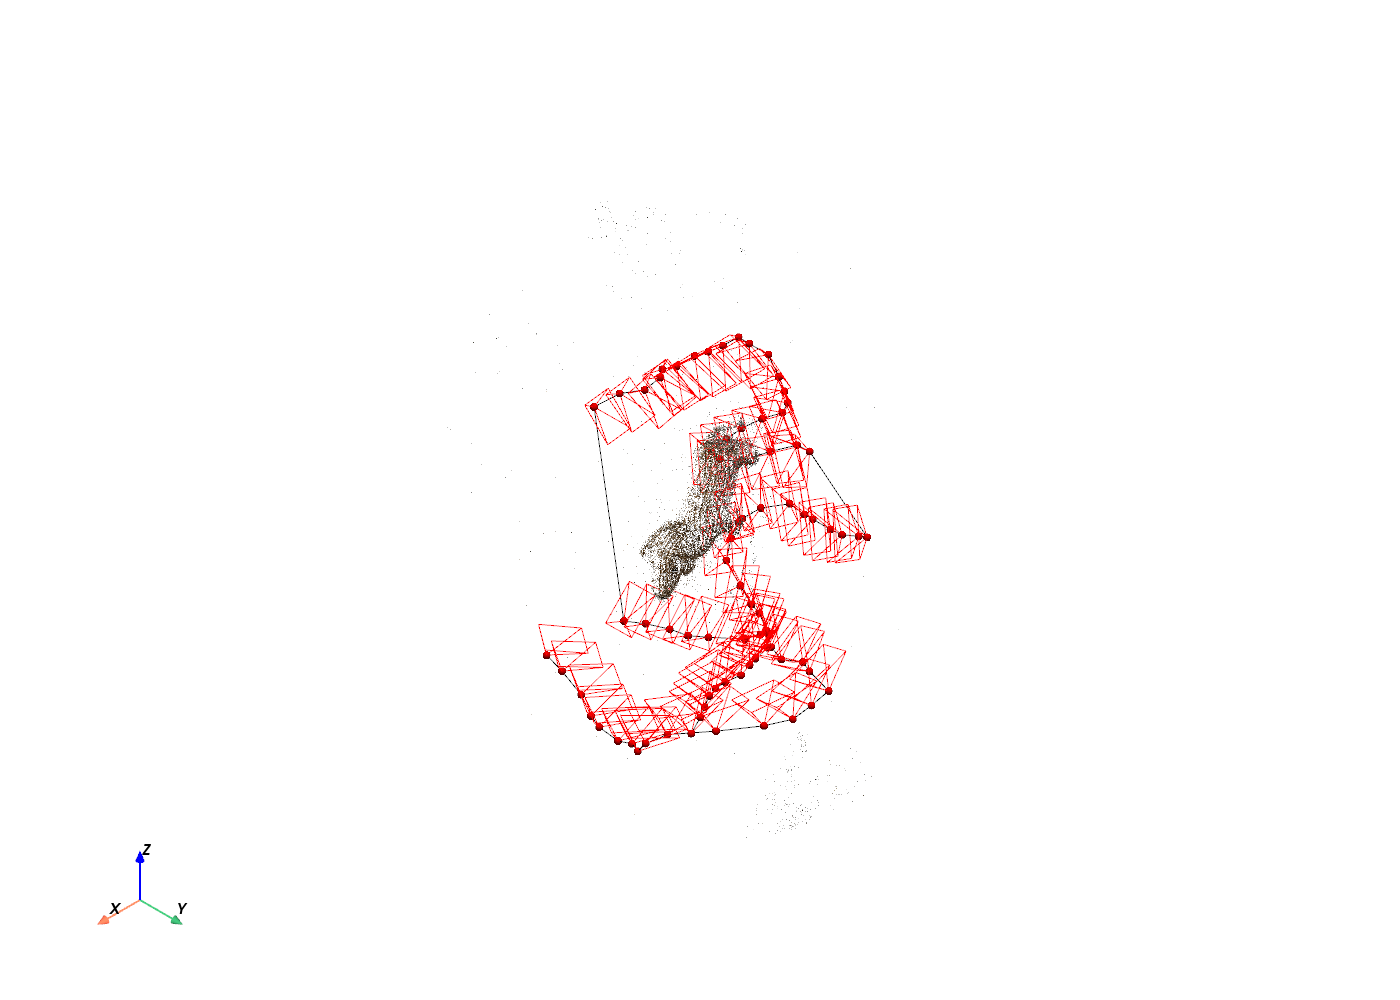
\includegraphics[width=0.78\linewidth]{fig_reconstruction.png}
\caption{Final reconstruction on the full \texttt{Doge} set: 78 registered camera
frusta (red), the registration-order trajectory (black), and the sparse cloud
(grey, the statue recognisable at centre). The trajectory's long leaps mark the
capture gaps; the four unregistered blocks appear as the empty arcs of the
walk-around.}
\label{fig:qual}
\end{figure}

\subsection{Scaling failures and fixes}
Pointing the working 20-frame pipeline at the full 169-image set exposed three
distinct failures, each diagnosed from a measured symptom.

\paragraph{The stall (coverage).} The run first stopped at 87/169 with whole
contiguous capture-time blocks empty. This was \emph{not} drift (the 2D--3D count
is combinatorial and cannot fall with pose error) and \emph{not} a disconnected
graph (17 unregistered images had $\ge 100$ verified inliers to a registered
image). The cause was the hard \texttt{break} above. Replacing it with a soft
stop, lowering the gates, and adding \texttt{\_extend\_tracks} were
\textbf{necessary but not sufficient}: coverage improved but the run still stalled
(\,$\sim$76/169\,), because the remaining blocks are real viewpoint
discontinuities, not loop behaviour.

\paragraph{Intrinsics (the largest quality fix).} Registered cameras were
initially low quality (PnP inlier ratios of a few percent). $\mathbf{K}$ had been
built with a hardcoded principal point $(800,600)$ and a focal assuming a
4:3, 2000-px-diagonal frame, whereas the Doge photos are 16:9 (native
$4000\times2256$, resized to $1600\times902$); $c_y$ was off by $\sim$149 px
($\approx$16\% of frame height), feeding a systematically wrong camera into every
PnP and triangulation. Deriving the focal from a 24\,mm-equivalent ($\to$1018.8
px) and auto-centring the principal point to $(799.5, 450.5)$ moved the median
reprojection error from \textbf{1.273 to 0.611 px} and made registrations
uniformly clean. We now persist $\mathbf{K}$ in \texttt{cameras.json} so
intrinsics are never again a forensic guess.

\paragraph{PnP inlier-ratio gate (quality).} An absolute inlier floor alone
accepts drifted poses that clear the floor (e.g.\ 37 inliers) while explaining
only 3--5\% of their correspondences. A second gate rejecting
$\text{inliers} < 0.30 \times \text{count}$ catches the opposite failure to the
floor. Together they moved the PnP inlier-ratio minimum from 0.03 to 0.31 and
eliminated all sub-0.30 registrations (vs.\ 53/98 before).

\subsection{Failure cases: why 91 images never register}
The 91 unregistered images form four contiguous capture-gap blocks (e.g.\ a
3.3\,s jump where the camera was repositioned). The natural hypothesis --- that
they are starved of correspondences --- is \emph{false}: probing each against the
final cloud, the rejected images have a median of $\sim$376 2D--3D footholds,
comfortably above the \texttt{min\_corr} floor. What fails is the geometry. Their
PnP inlier ratio is median \textbf{0.00} (max 0.19), whereas every registered image
sits at \textbf{$\ge 0.31$} (median 0.55). The two populations are cleanly
\emph{bimodal}, and the $0.30$ ratio gate falls in the empty $[0.19, 0.31]$ band
between them (Fig.~\ref{fig:pnp}). The matches exist but are geometrically
incompatible with the reconstructed pose, so no threshold setting can admit them
without admitting garbage --- the gate is robust, not arbitrarily placed. The fix
is structural: a separate model seeded on the rejected images registers a further
$+29$, confirming they form a coherent but disjoint cluster (§\ref{sec:disc}).

\begin{figure}[t]
\centering
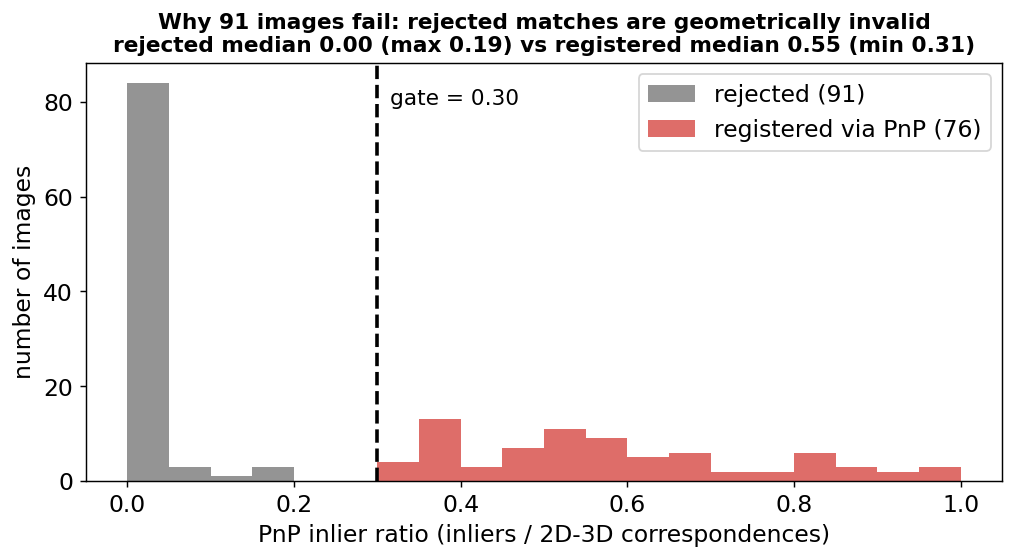
\includegraphics[width=0.7\linewidth]{fig_pnp_ratio_hist.png}
\caption{PnP inlier ratio for registered (red) vs.\ rejected (grey) images on the
full set. The distributions are bimodal with no overlap; the $0.30$ gate sits in
the empty gap. Rejected images are geometrically incompatible, not
correspondence-starved.}
\label{fig:pnp}
\end{figure}

A dead-end worth recording: loosening the Lowe ratio to 0.85 made coverage
\emph{worse} (18/169), because PnP does not re-verify matches with a fundamental
matrix the way the seed step does, so false correspondences poison it directly;
and raising the feature cap to 8000 was bit-identical, because SIFT finds
$\le 3363$ keypoints/image here, so the 4000 cap never bound. The weak bridges
reflect genuine low visual overlap across the capture gaps, not a tunable matcher
limit.

\section{Comparison with COLMAP}

We ran COLMAP~\citep{schoenberger2016colmap} (exhaustive matching, default pipeline) on the same images as each
of our two reconstruction attempts. On the full 169-image set COLMAP registers
\textbf{all 169} in a single model with 114\,220 sparse points in 5.3 min, versus
our 78/169 and 24\,587 points (Table~\ref{tab:colmap}). Its cloud is
$\sim$4.6$\times$ denser and it crosses the capture gaps our pipeline cannot.

\paragraph{The density gap is feature detection, not the engine.} The full-set
comparison confounds two effects --- coverage and density --- so we isolate density
on the 20-frame set, where \emph{both} systems register all 20 cameras. Even with
identical coverage COLMAP builds 22\,882 points to our 6\,412
(Fig.~\ref{fig:colmap}, $\sim$3.6$\times$). The cause is upstream: COLMAP's
detector finds $\sim$10\,673 keypoints/image against our SIFT's $\sim$2\,001
($\sim$5$\times$), and once the keypoint budget is accounted for our triangulation
efficiency (kept points per keypoint) is comparable. The density gap is therefore a
\emph{feature-extraction} gap, fixable by lowering the SIFT contrast threshold,
\emph{not} a limitation of our reconstruction engine.

\begin{table}[t]
\centering
\caption{Our pipeline vs.\ COLMAP on the full \texttt{Doge} set (169 images).}
\label{tab:colmap}
\begin{tabular}{lcccc}
\toprule
 & Registered & Sparse points & Median reproj.\ (px) & Wall-clock \\
\midrule
Ours   & 78/169  & 24\,587  & 0.611      & $\sim$5 min \\
COLMAP & 169/169 & 114\,220 & $\sim$1.0  & 5.3 min \\
\bottomrule
\end{tabular}
\end{table}

\begin{figure}[t]
\centering
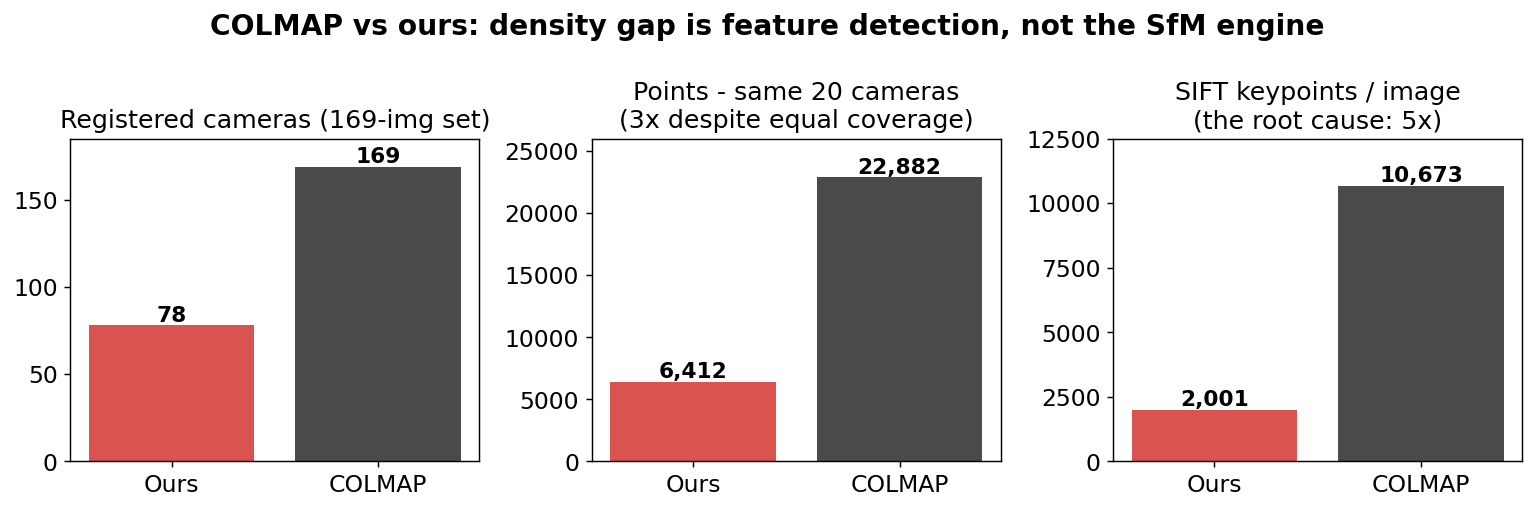
\includegraphics[width=\linewidth]{fig_colmap_compare.png}
\caption{COLMAP vs.\ ours. \emph{Left:} registered cameras on the full set
(coverage gap). \emph{Centre:} points on the same 20 cameras --- a density gap
that persists despite identical coverage. \emph{Right:} its root cause --- COLMAP's
detector finds $\sim$5$\times$ more keypoints per image.}
\label{fig:colmap}
\end{figure}

The \emph{coverage} difference has a specific mechanism, not merely ``COLMAP is
better'': COLMAP interleaves global bundle adjustment with retriangulation,
repeatedly refining all poses and points and then re-triangulating against the
improved poses, densifying the cloud until previously gap-isolated frames
accumulate enough valid structure to register. The load-bearing component is the
\emph{global optimisation} --- our own ablation (§\ref{sec:disc}) shows
retriangulation without it does nothing. Our single greedy forward pass has no
joint-refinement step, so a true low-overlap gap is terminal for us but bridgeable
for COLMAP.

\section{Discussion}
\label{sec:disc}

\subsection{What is missing to reach COLMAP-quality}

\paragraph{Bundle adjustment is the missing piece --- and we have direct evidence.}
We implemented retriangulation (re-triangulating existing tracks against the
current cloud) and ablated it. It made \emph{no} difference: 78 vs.\ 75 cameras and
24\,587 vs.\ 23\,420 points, within run-to-run noise (Fig.~\ref{fig:retri}). This
null result is informative rather than disappointing: re-triangulating against
poses we never refined cannot improve them, so the gain COLMAP extracts from
retriangulation is really a gain from the \emph{global bundle adjustment} it
interleaves. We never jointly refine poses and points, so small per-step errors
accumulate as drift --- the visible median (0.55\,px) vs.\ mean (1.04\,px)
reprojection gap --- and retriangulation has no refined geometry to exploit.
\textbf{Global BA is therefore the single largest missing piece}; only once it
exists does retriangulation become worthwhile.

\begin{figure}[t]
\centering
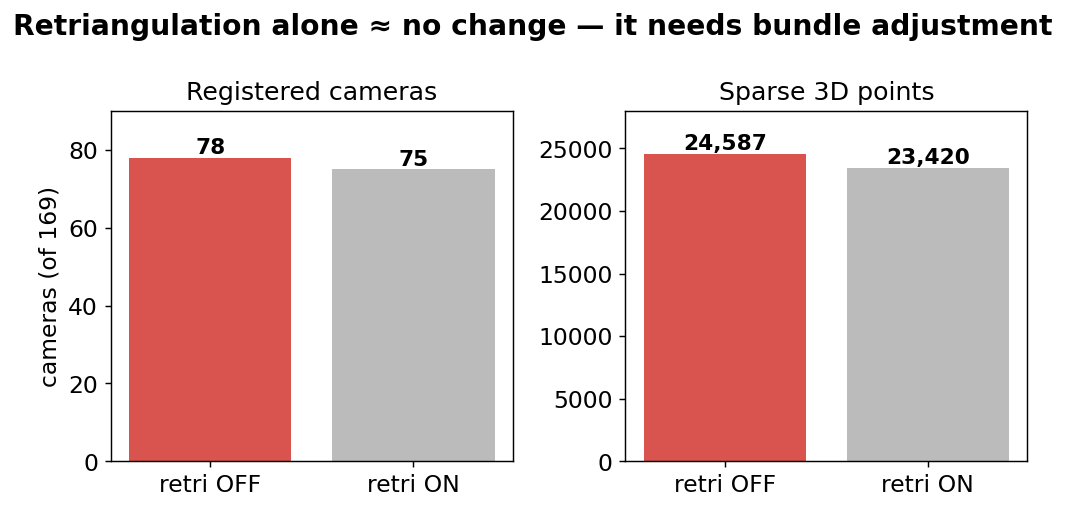
\includegraphics[width=0.72\linewidth]{fig_retri_ablation.png}
\caption{Retriangulation ablation on the full set. With no bundle adjustment to
refine the poses it triangulates against, retriangulation produces no improvement
in either cameras or points --- evidence that BA, not retriangulation, is the
load-bearing addition.}
\label{fig:retri}
\end{figure}

\paragraph{Two further capabilities.}
\begin{description}
  \item[Multi-model reconstruction with $\mathrm{Sim}(3)$ merging.] The coverage
  gap is a disjoint-cluster problem (Fig.~\ref{fig:pnp}): re-seed a fresh model
  from the best unregistered pair, grow it (a second model recovers $+29$ images
  here), and align models with a 7-DoF similarity (Umeyama~\citep{umeyama1991} + RANSAC) before a
  global BA closes the seam. This is the direct fix for the capture-gap blocks a
  single incremental model cannot cross.
  \item[Denser features.] As the COLMAP comparison showed, the density gap is upstream of the engine;
  a lower SIFT contrast threshold (or a learned detector) closes most of it.
\end{description}
We also lack track merging across loops (a point re-seen after the camera loops
back is duplicated, not merged) and per-image intrinsics (a single shared
$\mathbf{K}$ assumes one camera/resolution).

\subsection{First-principles reflection}
Our Week 1 study showed COLMAP itself failing on textureless surfaces, repetitive
patterns, low-overlap captures, and near-pure rotation. These are not COLMAP bugs
but consequences of the two hand-crafted primitives it shares with our pipeline.
\emph{SIFT} keys on local gradient structure, so a textureless or specular surface
yields no stable keypoints and a repetitive pattern yields many mutually ambiguous
ones; \emph{RANSAC on an epipolar/PnP model} can verify only what the matcher
proposes and degenerates when the motion is near-pure-rotation (no parallax,
essential matrix ill-conditioned) or the overlap is too low to outvote false
matches. Our pipeline exhibits sharper versions of the same modes: loosening the
Lowe ratio to 0.85 collapsed coverage to 18/169 (the false-match failure, since PnP
does not re-verify with a fundamental matrix), and our capture-gap blocks are
exactly the low-overlap case --- bimodal-bad PnP ratios (Fig.~\ref{fig:pnp}) where
the proposed matches are geometrically incompatible.

From first principles, then, two layers separate a robust system from where we are.
The first is the gap \emph{to} COLMAP: a purely incremental, locally-greedy
estimator has no global consistency constraint, so errors are neither bounded
(drift) nor repaired (gaps, duplicates); global bundle adjustment and multi-model
merging close this by optimising structure and motion jointly rather than committing
irreversibly to each local decision. The second is the gap \emph{past} COLMAP, and
it targets the Week 1 failures directly: because they originate in the correspondence
front-end, the principled remedy is \emph{learned} correspondence --- detectors and
matchers (e.g.\ SuperPoint~\citep{detone2018superpoint},
SuperGlue~\citep{sarlin2020superglue}, LoFTR~\citep{sun2021loftr}) that use semantic context to find
repeatable features on weak texture and to disambiguate repeated structure --- plus
motion priors and loop closure to constrain the degenerate-motion and revisited-scene
cases that no purely local, hand-crafted estimator can resolve.

\bibliographystyle{iclr2026_conference}
\bibliography{refs}

\appendix

\section{Iteration log: scaling from 20 to 169 images}
Each fix below was driven by a measured symptom, not a guess. Coverage is
\emph{cameras registered / 169}; quality is \emph{median per-observation
reprojection error}.

\begin{table}[h]
\centering
\small
\caption{Symptom $\to$ diagnosis $\to$ change $\to$ evidence for the full-set scaling.}
\begin{tabular}{p{2.4cm}p{3.4cm}p{3.0cm}p{3.2cm}}
\toprule
Symptom & Diagnosis & Change & Evidence \\
\midrule
Stall at 87/169, whole capture-time blocks empty &
Not drift (2D--3D count is combinatorial) and not a disconnected graph (17 unreg.\ images had $\ge$100 inliers to a reg.\ image); a hard \texttt{break} abandoned all remaining images at the first sub-floor pick &
Soft stop (reject-and-retry, cleared on any success); lower gates; add \texttt{\_extend\_tracks} to densify the frontier &
Necessary but not sufficient: $\sim$76/169 --- remaining blocks are real capture gaps \\
\addlinespace
Even registered cameras low quality (PnP ratios a few \%) &
$\mathbf{K}$ hardcoded for 4:3/2000px; data is 16:9, $c_y$ off by $\sim$149\,px ($\approx$16\% of height) &
Derive focal from 24\,mm-equiv $\to$1018.8\,px; auto-centre principal point; persist $\mathbf{K}$ in \texttt{cameras.json} &
Median reproj.\ \textbf{1.273$\to$0.611\,px}; registrations uniformly clean \\
\addlinespace
Drifted poses cleared the inlier \emph{floor} (e.g.\ 37 inliers, 3--5\% ratio) &
Absolute floor cannot reject many-point/low-fraction poses &
Add PnP inlier-\emph{ratio} gate ($<0.30\times$count) &
Ratio min 0.03$\to$0.31, median 0.27$\to$0.56; zero sub-0.30 (vs 53/98) \\
\addlinespace
Low-parallax points at garbage depth survive reproj.\ + cheirality &
Near-parallel rays slide along the ray at near-constant reprojection &
Per-point triangulation-angle floor ($\ge 2^\circ$) in \texttt{triangulate\_new\_points} &
Cleaner cloud at small coverage cost \\
\addlinespace
Weak bridges to stalled blocks ($\le$19 inliers) &
Hypothesis: more/looser matching lifts them &
Lowe 0.75$\to$0.85; features 4000$\to$8000 &
Worse (18/169) / bit-identical (SIFT finds $\le$3363 kp): dead end \\
\bottomrule
\end{tabular}
\end{table}

\noindent\textbf{Re-validation (correct $\mathbf{K}$ + final gates).} 78/169
cameras, 24\,587 points, median 0.611\,px / mean 1.031\,px; every registration
clean (PnP ratio min 0.31). The 91 unregistered images remain four contiguous
capture-gap blocks (\texttt{151332--151413}, \texttt{151432--151453}, the
\texttt{151517} two-frame island, \texttt{151549--151552}), confirming bad-$\mathbf{K}$
hurt \emph{quality} while the \emph{coverage} gap is independently the capture gaps.

\section{Group dynamics}
% TODO (author to complete): brief note on group dynamics over the last two weeks.
% Required item. State each member's contribution to the Week 4 system, experiments,
% report, and presentation in 2--3 sentences each.

\end{document}